\section{Info\-Area Class Reference}
\label{classInfoArea}\index{InfoArea@{InfoArea}}
{\tt \#include $<$infoarea.h$>$}

Inheritance diagram for Info\-Area:\begin{figure}[H]
\begin{center}
\leavevmode
\includegraphics[width=87pt]{classInfoArea__inherit__graph}
\end{center}
\end{figure}
Collaboration diagram for Info\-Area:\begin{figure}[H]
\begin{center}
\leavevmode
\includegraphics[width=121pt]{classInfoArea__coll__graph}
\end{center}
\end{figure}


\subsection{Detailed Description}
\begin{Desc}
\item[Author:]sonicat \end{Desc}




Definition at line 38 of file infoarea.h.\subsection*{Public Slots}
\begin{CompactItemize}
\item 
void {\bf slot\-Read\-List\-From\-Play\-List} (KURL::List playlist)
\item 
void {\bf Read\-List} ()
\item 
void {\bf slot\-Delete\-Items} ()
\item 
void {\bf slot\-Double\-Clicked} (QList\-View\-Item $\ast$item)
\item 
void {\bf slot\-Hadle\-Song\-Info} (int, int, QString, QString, QString)
\end{CompactItemize}
\subsection*{Signals}
\begin{CompactItemize}
\item 
void {\bf signal\-Read\-List} ()
\item 
void {\bf signal\-Remove\-List} (KURL::List removelist, {\bf HDASS\_\-ACTION\_\-TYPE} action)
\item 
void {\bf signal\-Play\-Item} (QString File\-Name)
\item 
void {\bf singal\-Play\-Item} ()
\end{CompactItemize}
\subsection*{Public Member Functions}
\begin{CompactItemize}
\item 
{\bf Info\-Area} ({\bf QWidget} $\ast$parent=0, const char $\ast$name=0)
\item 
void {\bf x\-Setup} ()
\item 
{\bf $\sim$Info\-Area} ()
\end{CompactItemize}
\subsection*{Public Attributes}
\begin{CompactItemize}
\item 
{\bf Skin\-Button} $\ast$ {\bf IABtn\-Volume\-Up}
\item 
{\bf Skin\-Button} $\ast$ {\bf IABtn\-Volume\-Down}
\item 
{\bf Skin\-Button} $\ast$ {\bf IABtn\-Play\-List\-Delete}
\item 
{\bf QWidget} $\ast$ {\bf m\_\-p\-Analyzer}
\item 
QList\-View $\ast$ {\bf Play\-List}
\item 
KURL::List {\bf curr\_\-list}
\end{CompactItemize}
\subsection*{Private Member Functions}
\begin{CompactItemize}
\item 
void {\bf Init\-Play\-List} ()
\item 
void {\bf Init\-Song\-Info} ()
\item 
void {\bf Show\-Song\-Info} (int m\_\-length, int m\_\-bitrate, QString m\_\-title, QString m\_\-artist, QString m\_\-album)
\end{CompactItemize}
\subsection*{Private Attributes}
\begin{CompactItemize}
\item 
QPixmap {\bf pix\-Background}
\item 
QPixmap $\ast$ {\bf Btn\-Graphic} [6]
\item 
QLabel $\ast$ {\bf Artist}
\item 
QLabel $\ast$ {\bf Album}
\item 
QLabel $\ast$ {\bf Length}
\item 
QLabel $\ast$ {\bf Year}
\item 
QLabel $\ast$ {\bf Title}
\item 
QLabel $\ast$ {\bf Bit\-Rate}
\end{CompactItemize}


\subsection{Constructor \& Destructor Documentation}
\index{InfoArea@{Info\-Area}!InfoArea@{InfoArea}}
\index{InfoArea@{InfoArea}!InfoArea@{Info\-Area}}
\subsubsection{\setlength{\rightskip}{0pt plus 5cm}Info\-Area::Info\-Area ({\bf QWidget} $\ast$ {\em parent} = 0, const char $\ast$ {\em name} = 0)}\label{classInfoArea_InfoAreaa0}




Definition at line 26 of file infoarea.cpp.

References x\-Setup().



\footnotesize\begin{verbatim}27  : QWidget(parent, name)
28 {
29   xSetup();
30 }
\end{verbatim}\normalsize 


Here is the call graph for this function:\begin{figure}[H]
\begin{center}
\leavevmode
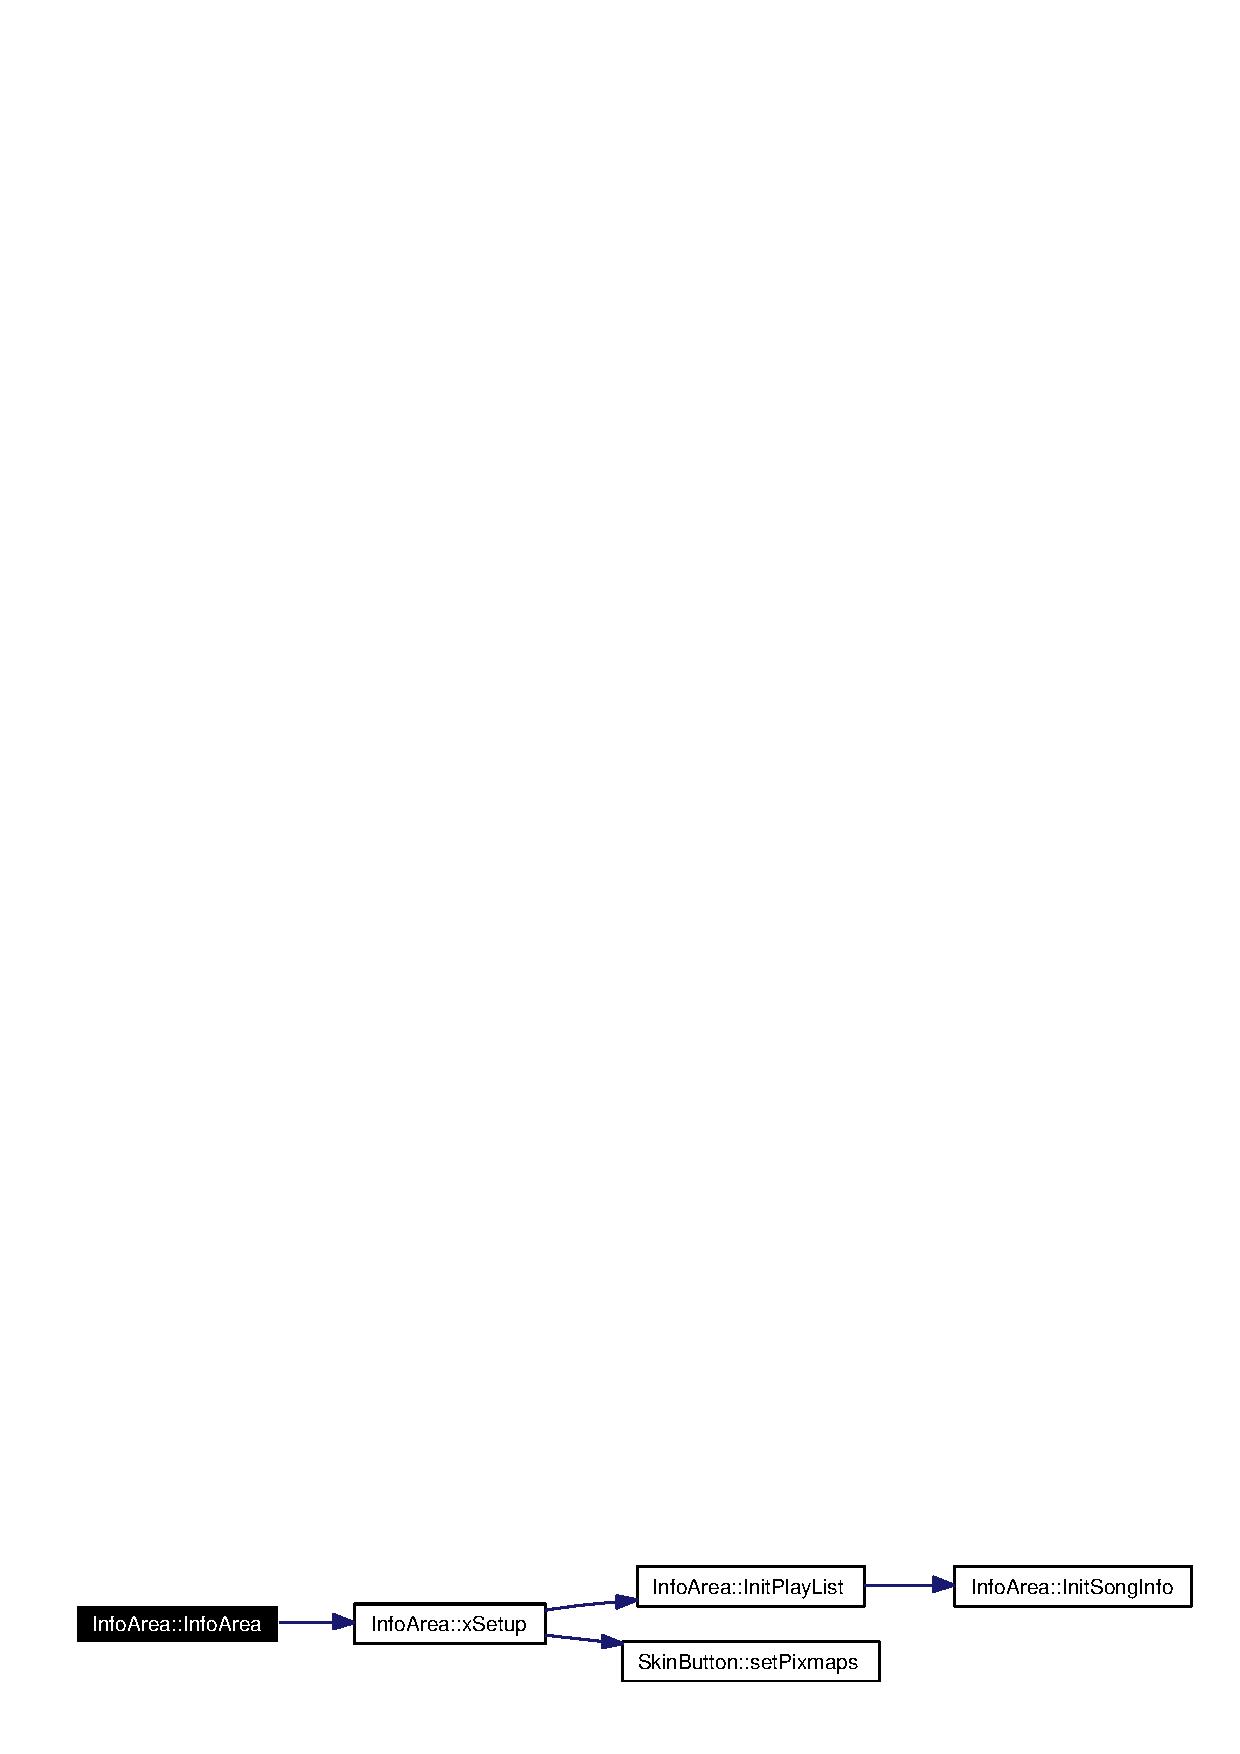
\includegraphics[width=286pt]{classInfoArea_InfoAreaa0_cgraph}
\end{center}
\end{figure}
\index{InfoArea@{Info\-Area}!~InfoArea@{$\sim$InfoArea}}
\index{~InfoArea@{$\sim$InfoArea}!InfoArea@{Info\-Area}}
\subsubsection{\setlength{\rightskip}{0pt plus 5cm}Info\-Area::$\sim${\bf Info\-Area} ()}\label{classInfoArea_InfoAreaa2}




Definition at line 33 of file infoarea.cpp.



\footnotesize\begin{verbatim}34 {
35 }
\end{verbatim}\normalsize 


\subsection{Member Function Documentation}
\index{InfoArea@{Info\-Area}!InitPlayList@{InitPlayList}}
\index{InitPlayList@{InitPlayList}!InfoArea@{Info\-Area}}
\subsubsection{\setlength{\rightskip}{0pt plus 5cm}void Info\-Area::Init\-Play\-List ()\hspace{0.3cm}{\tt  [private]}}\label{classInfoArea_InfoAread0}




Definition at line 77 of file infoarea.cpp.

References Init\-Song\-Info(), Play\-List, Read\-List(), and slot\-Double\-Clicked().

Referenced by x\-Setup().



\footnotesize\begin{verbatim}78 {
79   PlayList=new QListView(this);
80   PlayList->addColumn( "Items" );
81   PlayList->setColumnWidth(0,316);
82   PlayList->setRootIsDecorated( TRUE );
83   PlayList->setGeometry(35,60,316,420);
84   
85   QFont f( "Helvetica", 12, QFont::Bold );
86   PlayList->setFont( f );
87   
88   PlayList->show();
89   connect(PlayList,SIGNAL(doubleClicked ( QListViewItem * )),this,SLOT(slotDoubleClicked(QListViewItem* )));
90   ReadList();
91   InitSongInfo();
92   
93 }
\end{verbatim}\normalsize 


Here is the call graph for this function:\begin{figure}[H]
\begin{center}
\leavevmode
\includegraphics[width=148pt]{classInfoArea_InfoAread0_cgraph}
\end{center}
\end{figure}
\index{InfoArea@{Info\-Area}!InitSongInfo@{InitSongInfo}}
\index{InitSongInfo@{InitSongInfo}!InfoArea@{Info\-Area}}
\subsubsection{\setlength{\rightskip}{0pt plus 5cm}void Info\-Area::Init\-Song\-Info ()\hspace{0.3cm}{\tt  [private]}}\label{classInfoArea_InfoAread1}




Definition at line 141 of file infoarea.cpp.

References Artist, Bit\-Rate, and Title.

Referenced by Init\-Play\-List().



\footnotesize\begin{verbatim}142 {
143    Artist=new QLabel(this);
144    Artist->setPaletteBackgroundColor(QColor(255,255,255));
145    Artist->hide();
146    
147    Album=new QLabel(this);
148    Album->setPaletteBackgroundColor(QColor(255,255,255));
149    Album->hide();
150    
151    BitRate=new QLabel(this);
152    BitRate->setPaletteBackgroundColor(QColor(255,255,255));
153    BitRate->hide();
154    
155    Title=new QLabel(this);
156    Title->setPaletteBackgroundColor(QColor(255,255,255));
157    Title->hide();
158    
159    
160    Artist->move(420,210);
161    Album->move(420,240);
162    BitRate->move(420,270);
163    Title->move(580,270);
164    
165    QFont f( "Helvetica", 14, QFont::Bold );
166    
167    Artist->setFont( f );
168    Album->setFont( f );
169    Title->setFont( f );
170    BitRate->setFont( f );
171    
172 } 
\end{verbatim}\normalsize 
\index{InfoArea@{Info\-Area}!ReadList@{ReadList}}
\index{ReadList@{ReadList}!InfoArea@{Info\-Area}}
\subsubsection{\setlength{\rightskip}{0pt plus 5cm}void Info\-Area::Read\-List ()\hspace{0.3cm}{\tt  [slot]}}\label{classInfoArea_InfoAreai1}




Definition at line 112 of file infoarea.cpp.

References signal\-Read\-List().

Referenced by Init\-Play\-List(), and HDASS08::x\-Setup().



\footnotesize\begin{verbatim}113 {
114       emit signalReadList();
115 }
\end{verbatim}\normalsize 
\index{InfoArea@{Info\-Area}!ShowSongInfo@{ShowSongInfo}}
\index{ShowSongInfo@{ShowSongInfo}!InfoArea@{Info\-Area}}
\subsubsection{\setlength{\rightskip}{0pt plus 5cm}void Info\-Area::Show\-Song\-Info (int {\em m\_\-length}, int {\em m\_\-bitrate}, QString {\em m\_\-title}, QString {\em m\_\-artist}, QString {\em m\_\-album})\hspace{0.3cm}{\tt  [private]}}\label{classInfoArea_InfoAread2}




Definition at line 173 of file infoarea.cpp.



\footnotesize\begin{verbatim}174 {
175 
176 }
\end{verbatim}\normalsize 
\index{InfoArea@{Info\-Area}!signalPlayItem@{signalPlayItem}}
\index{signalPlayItem@{signalPlayItem}!InfoArea@{Info\-Area}}
\subsubsection{\setlength{\rightskip}{0pt plus 5cm}void Info\-Area::signal\-Play\-Item (QString {\em File\-Name})\hspace{0.3cm}{\tt  [signal]}}\label{classInfoArea_InfoAreal2}




Definition at line 141 of file infoarea.moc.

Referenced by slot\-Double\-Clicked().



\footnotesize\begin{verbatim}142 {
143     activate_signal( staticMetaObject()->signalOffset() + 2, t0 );
144 }
\end{verbatim}\normalsize 
\index{InfoArea@{Info\-Area}!signalReadList@{signalReadList}}
\index{signalReadList@{signalReadList}!InfoArea@{Info\-Area}}
\subsubsection{\setlength{\rightskip}{0pt plus 5cm}void Info\-Area::signal\-Read\-List ()\hspace{0.3cm}{\tt  [signal]}}\label{classInfoArea_InfoAreal0}




Definition at line 118 of file infoarea.moc.

Referenced by Read\-List().



\footnotesize\begin{verbatim}119 {
120     activate_signal( staticMetaObject()->signalOffset() + 0 );
121 }
\end{verbatim}\normalsize 
\index{InfoArea@{Info\-Area}!signalRemoveList@{signalRemoveList}}
\index{signalRemoveList@{signalRemoveList}!InfoArea@{Info\-Area}}
\subsubsection{\setlength{\rightskip}{0pt plus 5cm}void Info\-Area::signal\-Remove\-List (KURL::List {\em removelist}, {\bf HDASS\_\-ACTION\_\-TYPE} {\em action})\hspace{0.3cm}{\tt  [signal]}}\label{classInfoArea_InfoAreal1}




Definition at line 127 of file infoarea.moc.

Referenced by slot\-Delete\-Items().



\footnotesize\begin{verbatim}128 {
129     if ( signalsBlocked() )
130         return;
131     QConnectionList *clist = receivers( staticMetaObject()->signalOffset() + 1 );
132     if ( !clist )
133         return;
134     QUObject o[3];
135     static_QUType_ptr.set(o+1,&t0);
136     static_QUType_ptr.set(o+2,&t1);
137     activate_signal( clist, o );
138 }
\end{verbatim}\normalsize 
\index{InfoArea@{Info\-Area}!singalPlayItem@{singalPlayItem}}
\index{singalPlayItem@{singalPlayItem}!InfoArea@{Info\-Area}}
\subsubsection{\setlength{\rightskip}{0pt plus 5cm}void Info\-Area::singal\-Play\-Item ()\hspace{0.3cm}{\tt  [signal]}}\label{classInfoArea_InfoAreal3}




Definition at line 147 of file infoarea.moc.

Referenced by slot\-Double\-Clicked().



\footnotesize\begin{verbatim}148 {
149     activate_signal( staticMetaObject()->signalOffset() + 3 );
150 }
\end{verbatim}\normalsize 
\index{InfoArea@{Info\-Area}!slotDeleteItems@{slotDeleteItems}}
\index{slotDeleteItems@{slotDeleteItems}!InfoArea@{Info\-Area}}
\subsubsection{\setlength{\rightskip}{0pt plus 5cm}void Info\-Area::slot\-Delete\-Items ()\hspace{0.3cm}{\tt  [slot]}}\label{classInfoArea_InfoAreai2}




Definition at line 116 of file infoarea.cpp.

References curr\_\-list, em\_\-remove, Play\-List, and signal\-Remove\-List().

Referenced by x\-Setup().



\footnotesize\begin{verbatim}117 {
118         KURL::List remove_list;
119         int i=0;
120         HDASSPlayListItem *CurChild=(HDASSPlayListItem*)PlayList->firstChild();
121         for(KURL::List::ConstIterator remove_it = curr_list.begin();remove_it != curr_list.end();remove_it++,i++)
122         {
123                 if(CurChild->isSelected ())
124                 
125                 {
126                         remove_list <<(*remove_it).url();
127                 }
128                 CurChild=(HDASSPlayListItem*)CurChild->nextSibling();
129         }
130         emit signalRemoveList(remove_list,em_remove);
131 }
\end{verbatim}\normalsize 
\index{InfoArea@{Info\-Area}!slotDoubleClicked@{slotDoubleClicked}}
\index{slotDoubleClicked@{slotDoubleClicked}!InfoArea@{Info\-Area}}
\subsubsection{\setlength{\rightskip}{0pt plus 5cm}void Info\-Area::slot\-Double\-Clicked (QList\-View\-Item $\ast$ {\em item})\hspace{0.3cm}{\tt  [slot]}}\label{classInfoArea_InfoAreai3}




Definition at line 133 of file infoarea.cpp.

References signal\-Play\-Item(), and singal\-Play\-Item().

Referenced by Init\-Play\-List().



\footnotesize\begin{verbatim}134 {
135    HDASSPlayListItem *clickitem=(HDASSPlayListItem *)item;
136    qWarning("DoubleClikced");
137    emit signalPlayItem(clickitem->text(0));
138    emit singalPlayItem();
139  
140 }
\end{verbatim}\normalsize 
\index{InfoArea@{Info\-Area}!slotHadleSongInfo@{slotHadleSongInfo}}
\index{slotHadleSongInfo@{slotHadleSongInfo}!InfoArea@{Info\-Area}}
\subsubsection{\setlength{\rightskip}{0pt plus 5cm}void Info\-Area::slot\-Hadle\-Song\-Info (int, int, QString, QString, QString)\hspace{0.3cm}{\tt  [slot]}}\label{classInfoArea_InfoAreai4}




Definition at line 177 of file infoarea.cpp.

References Artist, Bit\-Rate, and Title.



\footnotesize\begin{verbatim}178 {
179    QString strArtist=QString("Artist :") +(m_artist.isEmpty()?QString(" No Info"):m_artist);
180    QString strTitle=(m_title.isEmpty()?QString(" No Info"):m_title);
181    QString strAlbum=QString("Album :") +(m_album.isEmpty()?QString(" No Info"):m_album);
182    
183    QFont f( "Helvetica", 14, QFont::Bold );
184    QFontMetrics fm(f);
185    
186    Artist->resize(fm.width(strArtist),fm.height());
187    Artist->setText(strArtist);
188    
189    Title->move(580-fm.width(strTitle)/2,Title->y());
190    Title->resize(fm.width(strTitle),fm.height());
191    Title->setText(strTitle);
192    
193    Album->resize(fm.width(strTitle),fm.height());
194    Album->setText(strAlbum);
195    
196    BitRate->setText(QString("BitRate : %1 ").arg(m_bitrate));
197     
198    //Artist->show();
199   // Album->show();
200    //BitRate->show();
201    Title->show();
202 
203    
204 }
\end{verbatim}\normalsize 
\index{InfoArea@{Info\-Area}!slotReadListFromPlayList@{slotReadListFromPlayList}}
\index{slotReadListFromPlayList@{slotReadListFromPlayList}!InfoArea@{Info\-Area}}
\subsubsection{\setlength{\rightskip}{0pt plus 5cm}void Info\-Area::slot\-Read\-List\-From\-Play\-List (KURL::List {\em playlist})\hspace{0.3cm}{\tt  [slot]}}\label{classInfoArea_InfoAreai0}




Definition at line 97 of file infoarea.cpp.

References curr\_\-list, and Play\-List.



\footnotesize\begin{verbatim}98 { 
99    curr_list=playlist;
100    //Clear ValueList
101    PlayList->clear();
102    
103    
104    for( KURL::List::ConstIterator it = playlist.begin();it != playlist.end();it++)
105    {
106     //Add to value list
107     qWarning((*it).fileName());
108      new HDASSPlayListItem( PlayList,(*it).fileName());
109    }
110 }
\end{verbatim}\normalsize 
\index{InfoArea@{Info\-Area}!xSetup@{xSetup}}
\index{xSetup@{xSetup}!InfoArea@{Info\-Area}}
\subsubsection{\setlength{\rightskip}{0pt plus 5cm}void Info\-Area::x\-Setup ()}\label{classInfoArea_InfoAreaa1}




Definition at line 37 of file infoarea.cpp.

References Btn\-Graphic, IABtn\-Play\-List\-Delete, IABtn\-Volume\-Down, IABtn\-Volume\-Up, Init\-Play\-List(), m\_\-p\-Analyzer, Skin\-Button::set\-Pixmaps(), and slot\-Delete\-Items().

Referenced by Info\-Area().



\footnotesize\begin{verbatim}38 {
39    //DAVID Setup Background;
40    pixBackground.load("/root/kde_application/hdass08/skin/InfoAreaBackground.png");
41    setBackgroundPixmap(pixBackground);
42    
43    //DAVID
44    m_pAnalyzer = new Sonogram( this );            
45    m_pAnalyzer->setGeometry( 417,144, 338,60 );
46    m_pAnalyzer->show();
47    
48    //DAVID Load BtnGraphic
49    BtnGraphic[0]=new QPixmap("/root/kde_application/hdass08/skin/InfoAreaBtn-VolumeUp.png");
50    BtnGraphic[1]=new QPixmap("/root/kde_application/hdass08/skin/InfoAreaBtn-VolumeUp-Active.png");
51    BtnGraphic[2]=new QPixmap("/root/kde_application/hdass08/skin/InfoAreaBtn-VolumeDown.png");
52    BtnGraphic[3]=new QPixmap("/root/kde_application/hdass08/skin/InfoAreaBtn-VolumeDown-Active.png");
53    BtnGraphic[4]=new QPixmap("/root/kde_application/hdass08/skin/InfoAreaBtn-PlayListDelete.png");
54    BtnGraphic[5]=new QPixmap("/root/kde_application/hdass08/skin/InfoAreaBtn-PlayListDelete-Active.png");
55    //DAVID Set Volume Buttons
56    IABtnVolumeUp=new SkinButton(this);
57    IABtnVolumeDown=new SkinButton(this);
58    IABtnPlayListDelete=new SkinButton(this);
59 
60    IABtnVolumeUp->setPixmaps(BtnGraphic[0],BtnGraphic[1]);
61    IABtnVolumeUp->setGeometry(418,38,60,60);
62    IABtnVolumeUp->show();
63    
64    IABtnVolumeDown->setPixmaps(BtnGraphic[2],BtnGraphic[3]);
65    IABtnVolumeDown->setGeometry(684,349,60,60);
66    IABtnVolumeDown->show();
67    
68    IABtnPlayListDelete->setPixmaps(BtnGraphic[4],BtnGraphic[5]);
69    IABtnPlayListDelete->setGeometry(346,477,42,42);
70    IABtnPlayListDelete->show();
71    connect(IABtnPlayListDelete,SIGNAL(clicked()),this,SLOT(slotDeleteItems()));
72    //DAVID Init PlayList Table
73    InitPlayList();
74    
75    
76 }
\end{verbatim}\normalsize 


Here is the call graph for this function:\begin{figure}[H]
\begin{center}
\leavevmode
\includegraphics[width=219pt]{classInfoArea_InfoAreaa1_cgraph}
\end{center}
\end{figure}


\subsection{Member Data Documentation}
\index{InfoArea@{Info\-Area}!Album@{Album}}
\index{Album@{Album}!InfoArea@{Info\-Area}}
\subsubsection{\setlength{\rightskip}{0pt plus 5cm}QLabel $\ast$ {\bf Info\-Area::Album}\hspace{0.3cm}{\tt  [private]}}\label{classInfoArea_InfoArear3}




Definition at line 64 of file infoarea.h.\index{InfoArea@{Info\-Area}!Artist@{Artist}}
\index{Artist@{Artist}!InfoArea@{Info\-Area}}
\subsubsection{\setlength{\rightskip}{0pt plus 5cm}QLabel$\ast$ {\bf Info\-Area::Artist}\hspace{0.3cm}{\tt  [private]}}\label{classInfoArea_InfoArear2}




Definition at line 64 of file infoarea.h.

Referenced by Init\-Song\-Info(), and slot\-Hadle\-Song\-Info().\index{InfoArea@{Info\-Area}!BitRate@{BitRate}}
\index{BitRate@{BitRate}!InfoArea@{Info\-Area}}
\subsubsection{\setlength{\rightskip}{0pt plus 5cm}QLabel $\ast$ {\bf Info\-Area::Bit\-Rate}\hspace{0.3cm}{\tt  [private]}}\label{classInfoArea_InfoArear7}




Definition at line 64 of file infoarea.h.

Referenced by Init\-Song\-Info(), and slot\-Hadle\-Song\-Info().\index{InfoArea@{Info\-Area}!BtnGraphic@{BtnGraphic}}
\index{BtnGraphic@{BtnGraphic}!InfoArea@{Info\-Area}}
\subsubsection{\setlength{\rightskip}{0pt plus 5cm}QPixmap$\ast$ {\bf Info\-Area::Btn\-Graphic}[6]\hspace{0.3cm}{\tt  [private]}}\label{classInfoArea_InfoArear1}




Definition at line 63 of file infoarea.h.

Referenced by x\-Setup().\index{InfoArea@{Info\-Area}!curr_list@{curr\_\-list}}
\index{curr_list@{curr\_\-list}!InfoArea@{Info\-Area}}
\subsubsection{\setlength{\rightskip}{0pt plus 5cm}KURL::List {\bf Info\-Area::curr\_\-list}}\label{classInfoArea_InfoAreao5}




Definition at line 49 of file infoarea.h.

Referenced by slot\-Delete\-Items(), and slot\-Read\-List\-From\-Play\-List().\index{InfoArea@{Info\-Area}!IABtnPlayListDelete@{IABtnPlayListDelete}}
\index{IABtnPlayListDelete@{IABtnPlayListDelete}!InfoArea@{Info\-Area}}
\subsubsection{\setlength{\rightskip}{0pt plus 5cm}{\bf Skin\-Button} $\ast$ {\bf Info\-Area::IABtn\-Play\-List\-Delete}}\label{classInfoArea_InfoAreao2}




Definition at line 45 of file infoarea.h.

Referenced by x\-Setup().\index{InfoArea@{Info\-Area}!IABtnVolumeDown@{IABtnVolumeDown}}
\index{IABtnVolumeDown@{IABtnVolumeDown}!InfoArea@{Info\-Area}}
\subsubsection{\setlength{\rightskip}{0pt plus 5cm}{\bf Skin\-Button} $\ast$ {\bf Info\-Area::IABtn\-Volume\-Down}}\label{classInfoArea_InfoAreao1}




Definition at line 45 of file infoarea.h.

Referenced by x\-Setup(), and HDASS08::x\-Setup().\index{InfoArea@{Info\-Area}!IABtnVolumeUp@{IABtnVolumeUp}}
\index{IABtnVolumeUp@{IABtnVolumeUp}!InfoArea@{Info\-Area}}
\subsubsection{\setlength{\rightskip}{0pt plus 5cm}{\bf Skin\-Button}$\ast$ {\bf Info\-Area::IABtn\-Volume\-Up}}\label{classInfoArea_InfoAreao0}




Definition at line 45 of file infoarea.h.

Referenced by x\-Setup(), and HDASS08::x\-Setup().\index{InfoArea@{Info\-Area}!Length@{Length}}
\index{Length@{Length}!InfoArea@{Info\-Area}}
\subsubsection{\setlength{\rightskip}{0pt plus 5cm}QLabel $\ast$ {\bf Info\-Area::Length}\hspace{0.3cm}{\tt  [private]}}\label{classInfoArea_InfoArear4}




Definition at line 64 of file infoarea.h.\index{InfoArea@{Info\-Area}!m_pAnalyzer@{m\_\-pAnalyzer}}
\index{m_pAnalyzer@{m\_\-pAnalyzer}!InfoArea@{Info\-Area}}
\subsubsection{\setlength{\rightskip}{0pt plus 5cm}{\bf QWidget}$\ast$ {\bf Info\-Area::m\_\-p\-Analyzer}}\label{classInfoArea_InfoAreao3}




Definition at line 46 of file infoarea.h.

Referenced by x\-Setup().\index{InfoArea@{Info\-Area}!pixBackground@{pixBackground}}
\index{pixBackground@{pixBackground}!InfoArea@{Info\-Area}}
\subsubsection{\setlength{\rightskip}{0pt plus 5cm}QPixmap {\bf Info\-Area::pix\-Background}\hspace{0.3cm}{\tt  [private]}}\label{classInfoArea_InfoArear0}




Definition at line 62 of file infoarea.h.\index{InfoArea@{Info\-Area}!PlayList@{PlayList}}
\index{PlayList@{PlayList}!InfoArea@{Info\-Area}}
\subsubsection{\setlength{\rightskip}{0pt plus 5cm}QList\-View$\ast$ {\bf Info\-Area::Play\-List}}\label{classInfoArea_InfoAreao4}




Definition at line 47 of file infoarea.h.

Referenced by Init\-Play\-List(), slot\-Delete\-Items(), and slot\-Read\-List\-From\-Play\-List().\index{InfoArea@{Info\-Area}!Title@{Title}}
\index{Title@{Title}!InfoArea@{Info\-Area}}
\subsubsection{\setlength{\rightskip}{0pt plus 5cm}QLabel $\ast$ {\bf Info\-Area::Title}\hspace{0.3cm}{\tt  [private]}}\label{classInfoArea_InfoArear6}




Definition at line 64 of file infoarea.h.

Referenced by Init\-Song\-Info(), and slot\-Hadle\-Song\-Info().\index{InfoArea@{Info\-Area}!Year@{Year}}
\index{Year@{Year}!InfoArea@{Info\-Area}}
\subsubsection{\setlength{\rightskip}{0pt plus 5cm}QLabel $\ast$ {\bf Info\-Area::Year}\hspace{0.3cm}{\tt  [private]}}\label{classInfoArea_InfoArear5}




Definition at line 64 of file infoarea.h.

The documentation for this class was generated from the following files:\begin{CompactItemize}
\item 
{\bf infoarea.h}\item 
{\bf infoarea.moc}\item 
{\bf infoarea.cpp}\end{CompactItemize}
